\documentclass[9pt]{extarticle}
\usepackage[utf8]{inputenc}
% column separation
\usepackage{multicol}
\usepackage[document]{ragged2e}
\usepackage{graphicx}
\setlength{\columnsep}{1cm}
\usepackage{tabularx}
\usepackage{cancel}
\usepackage{amsmath}
\usepackage{amsfonts}
\usepackage{siunitx}
\usepackage{pgfplots}
\usepackage[skins,theorems]{tcolorbox}
\newcommand*{\Scale}[2][4]{\scalebox{#1}{\ensuremath{#2}}}%
\tcbset{myinner/.style={no shadow,shrink tight,boxrule=0pt,frame style={opacity=0.25},interior style={opacity=0.5}}}
\usepgfplotslibrary{fillbetween}

\usepackage{filecontents}
\pgfplotsset{compat=1.16}
\usetikzlibrary{calc,arrows,fadings,positioning,angles,quotes,patterns}

\allowdisplaybreaks %% Fix for mega spaces

% page margins
\usepackage[a4paper, total={20cm, 25cm}]{geometry}

\title{Visual Data Analytics - Formulas}
\author{Adrian Castro}
\date{February 2021}

\begin{document}

\maketitle

\begin{multicols}{3}

%%
\section{General Knowledge}
%%
\textbf{Visualization Pipeline:}

$\bullet$ Data Acquisition \\
$\bullet$ Filtering/Enhancement (obtain useful data/cleaning) \\
$\bullet$ Visualization/Mapping (how to represent data) \\
$\bullet$ Rendering (generate 2D images/video)

\textbf{Indipendent Variables}: 2D/3D space, time \\
\textbf{Dependent Variables}: temperature, velocity

\textbf{Characteristics of data values}:

$\bullet$ Attribute types \\
$\bullet$ Domain \\
$\bullet$ Value range \\
$\bullet$ Dimension \\
$\bullet$ Error \& Uncertainty \\
$\bullet$ Physical Interpretration

\textbf{Qualitative data}: categorical, non-measurable, discrete \\
\textbf{Nominal data}: no natural ordering, membership \\
\textbf{Ordinal data}: natural ordering \\
\textbf{Categorical data}: values from fixed number or categories \\
\textbf{Scalar data}: if we can map from higher dimensional data to a lower dimensional data ($f(x): \mathbb{R}^n \rightarrow \mathbb{R}$) \\
\textbf{Tensor data}: multi-dimensional data \\

\section{Interpolation}

\textbf{ISOContours}: all points lying on the same line with the same values \\
\textbf{Goal of interpolation}: construct continuous function $f$ which approximates given values

\subsection{Radial Basis Functions}
Each point $(p_i, f_i)$ influences $f(x)$ based on distance: \\
$$r = \Vert p_i - x \Vert$$
$$f(x) = \sum_{i = 1}^{N} f_i \cdot \varphi(\Vert p_i - x \Vert)$$
$$\varphi(r) = e^{-r^2}$$

\textbf{Weighted radial basis functions}

$f(p_j)$ interpolates the value $f_j$

$$f(p_j) = \sum_{i = 1}^N w_i \cdot \varphi (\Vert p_i - p_j \Vert) = f_j$$

Yields a system of linear equations to be solved for $w_i$:

$$
    A = \begin{pmatrix}
        \varphi(\Vert p_1 - p_1 \Vert) & \cdots & \varphi(\Vert p_N - p_1 \Vert) \\
        \vdots                         & \ddots & \vdots                         \\
        \varphi(\Vert p_1 - p_N \Vert) & \cdots & \varphi(\Vert p_N - p_N \Vert)
    \end{pmatrix}
$$
$$
    W = \begin{bmatrix}
        w_1 \\ \vdots \\ w_N
    \end{bmatrix}
    F = \begin{bmatrix}
        f_1 \\ \vdots \\ f_N
    \end{bmatrix}
$$
$$W = A^{-1} \cdot F$$

\textbf{Drawbacks}: global influence of every sample, adding a new point requires solving the equation system, computationally expensive

\textbf{Inverse Distance Weighting}

\textbf{Assumption}: Nearby points are more similar than those further away.

$$f(x) = \sum_{i = 1}^N f_i \varphi(\Vert p_i - x \Vert)$$
$$d_i = \Vert p_i - x \Vert \hspace{1cm}
    \varphi(r) = \frac{\frac{1}{r^2}}{\sum_{i = 1}^N \frac{1}{d_i^2}}$$

\textbf{Adjusted formula}:
$$\sum_{i = 1}^N \frac{f_i}{\Vert p_i - x \Vert ^2} / \sum_{i = 1}^N \frac{1}{\Vert p_i - x \Vert ^2}$$

\textbf{Drawbacks}: still costly, still global influence of every sample

\subsection{Triangulation}
Giving up smooth, precise reconstruction in favor of speed

\textbf{Generating a Triangulation}

\textbf{Goals}: avoid long and thin triangles, maximize minimum angle in the triangulation, maximize $\frac{\text{radius of circle}}{\text{radius of circumcircle}}$

\textbf{Delaunay Triangulation}

\textbf{1}. Circumcircle does not contain another point of the set \\
\textbf{2}. Maximizes minimum angle of triangulation \\
\textbf{3}. Triangulation is unique for all but trivial cases

\textbf{Voronoi Diagram}

\begin{filecontents*}{voronoiPoints.dat}
    1.645370 0.643096
    -0.658113 1.655264
    -0.135778 -0.651569
\end{filecontents*}

\begin{filecontents*}{voronoiTriPoints.dat}
    -0.135778 -0.651569
    -0.658113 1.655264
    1.645370 0.643096
    -0.135778 -0.651569
\end{filecontents*}

\begin{filecontents*}{voronoi.dat}
    0.276155 0.654257
    -3.162349 -0.124321

    0.276155 0.654257
    1.694429 3.881949

    0.276155 0.654257
    2.349036 -2.197525

    0.276155 0.654257
    -3.162349 -0.124321
\end{filecontents*}

\begin{center}
    \begin{tikzpicture}[thick,scale=0.6, every node/.style={scale=0.6}]
        \begin{axis}[
                axis equal image,
                xtick=\empty,
                ytick=\empty,
                set layers
            ]
            \addplot [only marks, red] table {voronoiPoints.dat};
            \addplot [no markers, blue,name path=triangle] table {voronoiTriPoints.dat};
            \addplot [no markers, update limits=false,name path=lines] table {voronoi.dat};
            \node[below=2pt]
            at (axis cs:-0.135778,-0.651569)
            {$a$};
            \node[left=2pt]
            at (axis cs:-0.658113,1.655264)
            {$b$};
            \node[right=2pt]
            at (axis cs:1.645370,0.643096)
            {$c$};
            \clip[on layer=axis grid]
            (axis cs:-0.135778,-0.651569) --
            (axis cs:-0.658113,1.655264) --
            (axis cs:1.645370,0.643096) --
            (axis cs:-0.135778,-0.651569) -- cycle;
            \addplot fill between[
                    on layer=main,
                    of=triangle and lines,
                    split,
                    every segment no 0/.style={blue,fill opacity=0},
                    every segment no 1/.style={yellow,fill opacity=0.25},
                    every segment no 2/.style={red,fill opacity=0.25},
                    every segment no 3/.style={green,fill opacity=0.25},
                ];
        \end{axis}
    \end{tikzpicture}
\end{center}

Every \textbf{Voronoi Sample} ($a, b, c$) is a vertex of a \textbf{Delaunay} triangulation

\subsection{Interpolation Inside a Triangle}
\begin{center}
    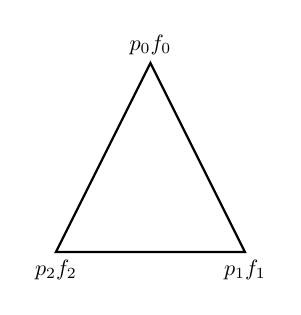
\begin{tikzpicture}[thick,scale=0.6, every node/.style={scale=0.8}]
        \draw (0,0) node[anchor=north]{$p_2 f_2$}
        -- (2,4) node[anchor=south]{$p_0 f_0$}
        -- (4,0) node[anchor=north]{$p_1 f_1$}
        -- cycle;
    \end{tikzpicture}
\end{center}

Find a function $f$ that interpolates $f_i$ at the point $p_i$ such that:

$$f(p_i) = f_i \hspace{1cm} i = 0, \cdots, N$$

Linear function:
$$f(x) = a + bx + cy$$

Where $a, b, c$ can be obtained with:

$$
    X = \begin{pmatrix}
        1 & x_0 & y_0 \\
        1 & x_1 & y_1 \\
        1 & x_2 & y_2 \\
    \end{pmatrix}
    A = \begin{bmatrix}
        a \\ b \\ c
    \end{bmatrix}
    F = \begin{bmatrix}
        f_0 \\ f_1 \\ f_2
    \end{bmatrix}
$$

$$A = X^{-1} \cdot F$$

\subsection{Baricentric Interpolation}

We want to have a smooth, continuous interpolation $\forall \alpha \in [0, 1]$

$$f(\alpha) = \alpha \cdot p_0 + (1 - \alpha) \cdot p_0$$

\begin{center}
    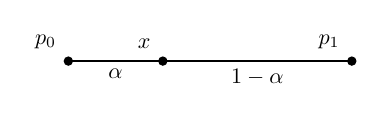
\begin{tikzpicture}[thick,scale=0.8, every node/.style={scale=0.8}]
        \tikzset{
            mydot/.style={
                    fill,
                    circle,
                    inner sep=1.5pt
                }
        }
        \path (0:4.5) coordinate (A) (0:1.5) coordinate (B) (0:0) coordinate (C);
        \draw (A)
        -- (B) node [midway, below]{$1 - \alpha$} -- (C) node [midway, below]{$\alpha$}  -- (A) -- cycle;
        \node[mydot,label={above left:$p_1$}] at (A) {};
        \node[mydot,label={above left:$x$}] at (B) {};
        \node[mydot,label={above left:$p_0$}] at (C) {};
        % \draw[|<->|] ($(A)!10mm!90:(C)$)--node[fill=white] {$z$} ($(C)!10mm!-90:(A)$);
    \end{tikzpicture}
\end{center}

$$\alpha_0 = A_0 / A , \ \alpha_1 = A_1 / A , \ \alpha_2 = A_2 / A$$
Where $A =$ area of the triangle
$$x = \alpha_0 p_0 + \alpha_1 p_1 + \alpha_2 p_2$$
$$\alpha_0 + \alpha_1 + \alpha_2 = 1$$

If $\alpha_i$ are known, then $f(x)$ can be interpolated from values $f_i$ at the vertices via:

$$f(x) = \alpha_0 f_0 + \alpha_1 f_1 + (1 - \alpha_0 - \alpha1) \cdot f_2$$

Given a point $Q$ we can find $\alpha$ by solving the linear system:

$$P = \begin{pmatrix}
        p_{0x} & p_{1x} & p_{2x} \\
        p_{0y} & p_{1y} & p_{2y} \\
        1      & 1      & 1      \\
    \end{pmatrix}$$
$$A = \begin{bmatrix}
        \alpha_0 \\ \alpha_1 \\ \alpha_2
    \end{bmatrix} X = \begin{bmatrix}
        Q_x \\ Q_y \\ 1
    \end{bmatrix}$$

$$A = P^{-1} \cdot X$$

\subsection{Scalar Interpolation}
Formula of tetrahedron:
$$f(x) = a + bx + cy + dz$$

\begin{center}
    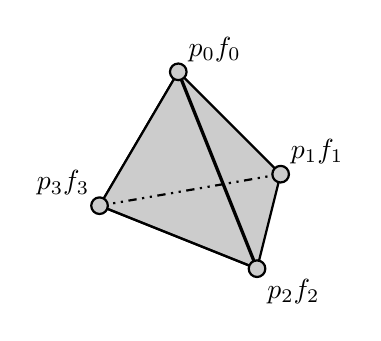
\begin{tikzpicture}

        \coordinate (a) at (4,2.5);
        \coordinate (b) at (3,.8);
        \coordinate (c) at (5,0);
        \coordinate (d) at (5.3,1.2);

        \draw[thick, fill=black!10] (a) -- (b) -- cycle;
        \draw[thick, fill=black!20] (a) -- (b) -- (c) -- (d) -- cycle;
        \draw[thick, fill=black!30] (b) -- (c) -- cycle;
        \draw[very thick] (a) -- (c);
        \draw[thick, dash dot dot] (b) -- (d);

        \fill[black!20, draw=black, thick] (a) circle (3pt) node[black, above right] {$p_0 f_0$};
        \fill[black!20, draw=black, thick] (b) circle (3pt) node[black, above left] {$p_3 f_3$};
        \fill[black!20, draw=black, thick] (c) circle (3pt) node[black, below right] {$p_2 f_2$};
        \fill[black!20, draw=black, thick] (d) circle (3pt) node[black, above right] {$p_1 f_1$};

    \end{tikzpicture}
\end{center}

Can get values $a, b, c, d$ by solving linear system:

$$X = \begin{pmatrix}
        1 & x_0 & y_0 & z_0 \\
        1 & x_1 & y_1 & z_1 \\
        1 & x_2 & y_2 & z_2 \\
        1 & x_3 & y_3 & z_3 \\
    \end{pmatrix}$$
$$A = \begin{bmatrix}
        a \\ b \\ c \\ d
    \end{bmatrix} F = \begin{bmatrix}
        f_0 \\ f_1 \\ f_2 \\ f_3
    \end{bmatrix}$$

$$A = X^{-1} \cdot F$$

\textbf{Computing Gradient of Scalar Field}

The gradient in a scalar field $f(x)$:
$$\nabla f(x) = \Scale[1.3]{\begin{pmatrix}
            \frac{\delta f(x)}{\delta x} \\
            \frac{\delta f(x)}{\delta y} \\
            \frac{\delta f(x)}{\delta z} \\
        \end{pmatrix}}$$

In the case of a tetrahedron with function the gradient is always constant:
$$f(x) = a + bx + cy + dz$$
$$\nabla f(x) = \Scale[1.3]{\begin{pmatrix}
            \frac{\delta f(x)}{\delta x} \\
            \frac{\delta f(x)}{\delta y} \\
            \frac{\delta f(x)}{\delta z} \\
        \end{pmatrix} = \begin{bmatrix}
            b \\ c \\ d
        \end{bmatrix}}$$

\subsection{Piece-Wise Linear Interpolation}

For data points $(x_0, y_0), \cdots, (x_N, y_N)$ \\
Evaluate
$$f(x) = (1 - \alpha)y_i + \alpha y_i$$
$$\text{where: } \alpha = \frac{x - x_1}{x_{i+1} - x_i}$$

\textbf{Bilinear Interpolation}

\begin{align*}
    f(\alpha, \beta) = & \tcbhighmath[myinner, colback=orange!50!white]{f_{ij} \cdot (1 - \alpha)(1 - \beta)} + \\
                       & \tcbhighmath[myinner, colback=blue!20!white]{f_{i+i, j} \cdot \alpha (1 - \beta)} +    \\
                       & \tcbhighmath[myinner, colback=violet!20!white]{f_{i, j+1} \cdot (1 - \alpha) \beta} +  \\
                       & \tcbhighmath[myinner, colback=green!20!white]{f_{i+1, j+1} \cdot \alpha \beta}
\end{align*}

\begin{center}
    \begin{tikzpicture}
        \coordinate (1) at (0,0);
        \coordinate (2) at (4,0);
        \coordinate (3) at (4,4);
        \coordinate (4) at (0,4);
        \fill (1) circle (1pt) node [left] {$\tcbhighmath[myinner, colback=orange!50!white]{f_{ij}}$};
        \fill (2) circle (1pt) node [right] {$\tcbhighmath[myinner, colback=blue!20!white]{f_{i + 1, j}}$};
        \fill (3) circle (1pt) node [above] {$\tcbhighmath[myinner, colback=green!20!white]{f_{i+1, j+1}}$};
        \fill (4) circle (1pt) node [above] {$\tcbhighmath[myinner, colback=violet!20!white]{f_{i, j+1}}$};
        \coordinate (5) at ($(1)!.4!(2)$);
        \fill (5) circle (1pt) node [below] {$\alpha$};
        \coordinate (6) at ($(2)!.4!(3)$);
        \fill (6) circle (1pt) node [right] {$\beta$};

        \coordinate (7) at ($(3)!.6!(4)$);

        \coordinate (8) at ($(1)!.4!(4)$);
        \coordinate (9) at ($(1)!.4!(3)$);
        \fill ($(1)!.4!(3)$) circle (1pt) node [above right] {$f$};

        \node[text width=15mm] at (0.8, 3) {$\tcbhighmath[myinner, colback=blue!20!white]{\alpha \cdot (1 - \beta)}$};
        \node[text width=15mm] at (1, 1) {$\tcbhighmath[myinner, colback=green!20!white]{\alpha \cdot \beta}$};
        \node[text width=20mm] at (2.6, 3) {$\tcbhighmath[myinner, colback=orange!50!white]{(1 - \alpha) \cdot (1 - \beta)}$};
        \node[text width=15mm] at (3, 1) {$\tcbhighmath[myinner, colback=violet!20!white]{(1 - \alpha) \cdot \beta}$};

        \draw (1)--(2)--(3)--(4)-- cycle;
        \draw (5)--(7);
        \draw (6)--(8);
    \end{tikzpicture}
\end{center}

\textbf{Asymptotic Decider}

\textbf{Hyperbola form}:
$$f(\alpha, \beta) = \gamma (\alpha - \alpha_0)(\beta - \beta_0) + \delta$$
$$\text{where }\delta\text{ is the value at point } (\alpha_0, \beta_0)$$

\begin{center}
    \begin{tikzpicture}
        \coordinate (1) at (0,0);
        \coordinate (2) at (4,0);
        \coordinate (3) at (4,4);
        \coordinate (4) at (0,4);
        \fill (1) circle (1pt) node [left] {$\tcbhighmath[myinner, colback=orange!50!white]{f_{ij}}$};
        \fill (2) circle (1pt) node [right] {$\tcbhighmath[myinner, colback=blue!20!white]{f_{i + 1, j}}$};
        \fill (3) circle (1pt) node [above] {$\tcbhighmath[myinner, colback=green!20!white]{f_{i + 1, j + 1}}$};
        \fill (4) circle (1pt) node [above] {$\tcbhighmath[myinner, colback=violet!20!white]{f_{i, j+1}}$};
        \coordinate (5) at ($(1)!.4!(2)$);
        \fill (5) circle (1pt) node [below] {$\alpha_0$};
        \coordinate (6) at ($(2)!.4!(3)$);
        \fill (6) circle (1pt) node [right] {$\beta_0$};

        \coordinate (7) at ($(3)!.6!(4)$);

        \coordinate (8) at ($(1)!.4!(4)$);
        \coordinate (9) at ($(1)!.4!(3)$);
        \fill ($(1)!.4!(3)$) circle (1pt) node [above right] {$(\alpha_0, \beta_0)$};

        \draw (1)--(2)--(3)--(4)-- cycle;
        \draw (5)--(7);
        \draw (6)--(8);
    \end{tikzpicture}
\end{center}

Transform to \textbf{hyperbola form}:

$$f(\alpha, \beta) = A\alpha + B\beta + C\alpha\beta + D$$
\begin{align*}
    A        & = \tcbhighmath[myinner, colback=blue!20!white]{f_{i + 1, j}} - \tcbhighmath[myinner, colback=orange!50!white]{f_{ij}}                                                                                                                                          \\
    B        & = \tcbhighmath[myinner, colback=violet!20!white]{f_{i, j+1}} - \tcbhighmath[myinner, colback=orange!50!white]{f_{ij}}                                                                                                                                          \\
    C        & = \tcbhighmath[myinner, colback=orange!50!white]{f_{ij}} - \tcbhighmath[myinner, colback=violet!20!white]{f_{i, j+1}} - \tcbhighmath[myinner, colback=blue!20!white]{f_{i + 1, j}} + \tcbhighmath[myinner, colback=green!20!white]{f_{i + 1, j + 1}}           \\
    D        & = \tcbhighmath[myinner, colback=orange!50!white]{f_{ij}}                                                                                                                                                                                                       \\
    \delta   & = (\tcbhighmath[myinner, colback=orange!50!white]{f_{ij}} \cdot \tcbhighmath[myinner, colback=green!20!white]{f_{i + 1, j + 1}} - \tcbhighmath[myinner, colback=blue!20!white]{f_{i + 1, j}} \cdot \tcbhighmath[myinner, colback=violet!20!white]{f_{i, j+1}}) \\
    \alpha_0 & = -B/C                                                                                                                                                                                                                                                         \\
    \beta_0  & = -A/C                                                                                                                                                                                                                                                         \\
    \gamma   & = C
\end{align*}

\subsection{Marching Squares}
Algorithm used to compute isolines on a 2D surface, given a grid of values. \\
\textbf{Step 1:} mark all the data with:
\begin{align*}
    \text{value} >= \text{isovalue: } & + \\
    \text{value} < \text{isovalue: }  & -
\end{align*}
\textbf{Step 2:} 16 different combinations, but we are interested in 4 base cases:
\begin{center}
    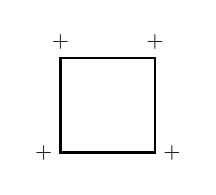
\begin{tikzpicture}[thick,scale=0.3, every node/.style={scale=0.8}]
        \coordinate (1) at (0,0);
        \coordinate (2) at (4,0);
        \coordinate (3) at (4,4);
        \coordinate (4) at (0,4);
        \fill (1) circle (1pt) node [left] {$+$};
        \fill (2) circle (1pt) node [right] {$+$};
        \fill (3) circle (1pt) node [above] {$+$};
        \fill (4) circle (1pt) node [above] {$+$};
        \coordinate (5) at ($(1)!.4!(2)$);
        % \fill (5) circle (1pt) node [below] {$\alpha_0$};
        \coordinate (6) at ($(2)!.4!(3)$);
        % \fill (6) circle (1pt) node [right] {$\beta_0$};

        \coordinate (7) at ($(3)!.6!(4)$);

        \coordinate (8) at ($(1)!.4!(4)$);
        \coordinate (9) at ($(1)!.4!(3)$);
        % \fill ($(1)!.4!(3)$) circle (1pt) node [above right] {$(\alpha_0, \beta_0)$};

        \draw (1)--(2)--(3)--(4)-- cycle;
        % \draw (5)--(7);
        % \draw (6)--(8);
    \end{tikzpicture}
    \qquad %
    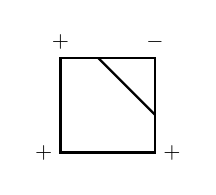
\begin{tikzpicture}[thick,scale=0.3, every node/.style={scale=0.8}]
        \coordinate (1) at (0,0);
        \coordinate (2) at (4,0);
        \coordinate (3) at (4,4);
        \coordinate (4) at (0,4);
        \fill (1) circle (1pt) node [left] {$+$};
        \fill (2) circle (1pt) node [right] {$+$};
        \fill (3) circle (1pt) node [above] {$-$};
        \fill (4) circle (1pt) node [above] {$+$};
        \coordinate (5) at ($(1)!.4!(2)$);
        % \fill (5) circle (1pt) node [below] {$\alpha_0$};
        \coordinate (6) at ($(2)!.4!(3)$);
        % \fill (6) circle (1pt) node [right] {$\beta_0$};

        \coordinate (7) at ($(3)!.6!(4)$);

        \coordinate (8) at ($(1)!.4!(4)$);
        \coordinate (9) at ($(1)!.4!(3)$);
        % \fill ($(1)!.4!(3)$) circle (1pt) node [above right] {$(\alpha_0, \beta_0)$};

        \draw (1)--(2)--(3)--(4)-- cycle;
        % \draw (5)--(7);
        \draw (6)--(7);
    \end{tikzpicture}

\end{center}

\begin{center}
    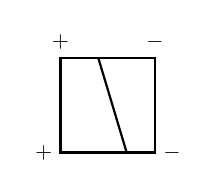
\begin{tikzpicture}[thick,scale=0.3, every node/.style={scale=0.8}]
        \coordinate (1) at (0,0);
        \coordinate (2) at (4,0);
        \coordinate (3) at (4,4);
        \coordinate (4) at (0,4);
        \fill (1) circle (1pt) node [left] {$+$};
        \fill (2) circle (1pt) node [right] {$-$};
        \fill (3) circle (1pt) node [above] {$-$};
        \fill (4) circle (1pt) node [above] {$+$};
        \coordinate (5) at ($(1)!.7!(2)$);
        \coordinate (6) at ($(2)!.4!(3)$);

        \coordinate (7) at ($(3)!.6!(4)$);

        \coordinate (8) at ($(1)!.4!(4)$);
        \coordinate (9) at ($(1)!.4!(3)$);
        % \fill ($(1)!.4!(3)$) circle (1pt) node [above right] {$(\alpha_0, \beta_0)$};

        \draw (1)--(2)--(3)--(4)-- cycle;
        \draw (5)--(7);
        % \draw (6)--(8);
    \end{tikzpicture}
\end{center}

In the last case, we have ambiguity, which can be resolved in two ways: \\
$\bullet$ midpoint decider:
$$f_{center} = \frac{1}{4} (f_{ij} + f_{i + 1, j} + f_{i, j + 1} + f_{i + 1, j + 1})$$
$\bullet$ if midpoint decider is right in the middle, hence the ambiguity is still there, we can use the \textbf{asymptotic decider} previously defined as:

$$f(\alpha, \beta) = \gamma (\alpha - \alpha_0)(\beta - \beta_0) + \delta$$

\begin{center}
    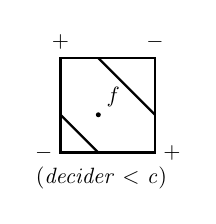
\begin{tikzpicture}[thick,scale=0.3, every node/.style={scale=0.8}]
        \coordinate (1) at (0,0);
        \coordinate (2) at (4,0);
        \coordinate (3) at (4,4);
        \coordinate (4) at (0,4);
        \fill (1) circle (1pt) node [left] {$-$};
        \fill (2) circle (1pt) node [right] {$+$};
        \fill (3) circle (1pt) node [above] {$-$};
        \fill (4) circle (1pt) node [above] {$+$};
        \coordinate (5) at ($(1)!.4!(2)$);
        \coordinate (6) at ($(2)!.4!(3)$);

        \coordinate (7) at ($(3)!.6!(4)$);

        \coordinate (8) at ($(1)!.4!(4)$);
        \coordinate (9) at ($(1)!.4!(3)$);
        \fill ($(1)!.4!(3)$) circle (3pt) node [above right] {$f$};

        \draw (1)--(2)--(3)--(4)-- cycle;
        \draw (6)--(7);
        \draw (8)--(5);
        \node at (2.5, -0.3, 2) {(\textit{decider} $<$ \textit{c})};
    \end{tikzpicture}
    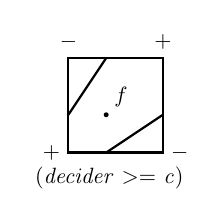
\begin{tikzpicture}[thick,scale=0.3, every node/.style={scale=0.8}]
        \coordinate (1) at (0,0);
        \coordinate (2) at (4,0);
        \coordinate (3) at (4,4);
        \coordinate (4) at (0,4);
        \fill (1) circle (1pt) node [left] {$+$};
        \fill (2) circle (1pt) node [right] {$-$};
        \fill (3) circle (1pt) node [above] {$+$};
        \fill (4) circle (1pt) node [above] {$-$};
        \coordinate (5) at ($(1)!.4!(2)$);
        % \fill (5) circle (1pt) node [below] {$\alpha_0$};
        \coordinate (6) at ($(2)!.4!(3)$);
        % \fill (6) circle (1pt) node [right] {$\beta_0$};

        \coordinate (7) at ($(3)!.6!(4)$);

        \coordinate (8) at ($(1)!.4!(4)$);
        \coordinate (9) at ($(1)!.4!(3)$);
        \fill ($(1)!.4!(3)$) circle (3pt) node [above right] {$f$};

        \draw (1)--(2)--(3)--(4)-- cycle;
        % \draw (5)--(7);
        \draw (5)--(6);
        \draw (7)--(8);
        \node at (2.5, -0.3, 2) {(\textit{decider} $>=$ \textit{c})};
    \end{tikzpicture}
\end{center}

\section{Phong Illumination Model}
Components: \\
$\bullet$ \textbf{Ambient Light}: background light, constant everywhere \\
$\bullet$ \textbf{Diffuse Reflector}: reflects equally into all directions \\
$\bullet$ \textbf{Specular Reflector}: reflects mostly into the mirror direction

\subsection{Lighting}

$$C = K_a C_a O_d$$
\begin{align*}
    K_a & : \text{ambient reflection coefficient }\in [0,1] \\
    C_a & : \text{color of the ambient light}               \\
    O_a & : \text{object color}
\end{align*}

\subsection{Diffuse Reflection}

\begin{center}
    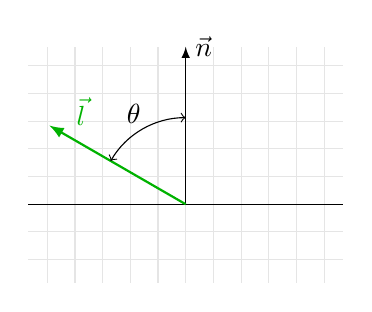
\begin{tikzpicture}[line/.style={>=latex}]
        \coordinate (V1) at (1, 1.3);
        \coordinate (V2) at (-1.6, 0.4);
        \coordinate (V3) at ($(V1) + (V2)$);
        \coordinate (V4) at ($1*(V1)$);
        \coordinate (O);

        \draw[step=10pt, color=black!10] (-2, -1) grid (2, 2);
        \draw[-, line] (-2, 0) -- node [below, very near end] {} (2, 0);
        \draw[->, line] (0, 0) -- ({2*cos(90)}, {2*sin(90)}) node[above right, very near end] {$\vec{n}$} coordinate (n);
        \draw[->, line, color=green!70!black, thick] (0, 0) -- ({2*cos(150)}, {2*sin(150)}) node[above right, very near end] {$\vec{l}$} coordinate (l);
        \pic [draw, <->, angle radius=11mm, angle eccentricity=1.2, "$\theta$"] {angle = n--O--l};
    \end{tikzpicture}
\end{center}

$$C = K_d C_p O_d \cdot \cos{\theta}$$
$$\cos{\theta} = \frac{\vec{n} \cdot \vec{l}}{\vert \vec{n} \vert \cdot \vert \vec{l} \vert}$$
\begin{align*}
    K_d          & : \text{diffuse reflection coefficient }\in [0, 1]                 \\
    C_p          & : \text{color of point of light}                                   \\
    O_d          & : \text{object color}                                              \\
    \cos{\theta} & : \text{angle between light vector } \vec{l}  \text{ and } \vec{n} \\
\end{align*}

\textbf{Reminder}:
$$\vert \vec{v} \vert = \sqrt{(v_0)^2 + \cdots + (v_n)^2}$$

\subsection{Specular Reflection}

$$C = K_s C_p O_d \cdot \cos^n{\varphi}$$
$$\cos{\varphi} = \frac{\vec{r}\cdot \vec{v}}{\vert \vec{r} \vert \cdot \vert \vec{v} \vert}$$
$$\vec{r} = 2 \cdot (\frac{\vec{n} \cdot \vec{l}}{\vert \vec{n} \vert \cdot \vert \vec{l} \vert}) \cdot \frac{\vec{n}}{\vert \vec{n} \vert} - \frac{\vec{l}}{\vert \vec{l} \vert}$$

\begin{align*}
    K_s             & : \text{specular reflection coefficient }\in [0, 1] \\
    C_p             & : \text{color of point of light}                    \\
    O_d             & : \text{object color}                               \\
    \cos^n{\varphi} & : \text{angle between reflected light ray } \vec{r} \\
                    & \text{\ \ \ and the vector to the viewer } \vec{v}  \\
    (\cdots)^n      & : \text{shininess factor (extent of highlight)}     \\
\end{align*}

\begin{center}
    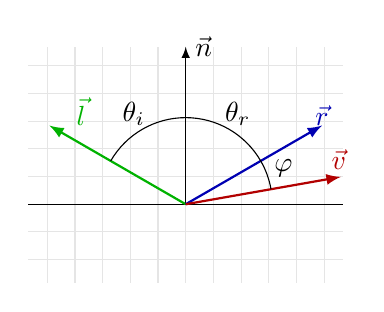
\begin{tikzpicture}[line/.style={>=latex}]
        \coordinate (V1) at (1, 1.3);
        \coordinate (V2) at (-1.6, 0.4);
        \coordinate (V3) at ($(V1) + (V2)$);
        \coordinate (V4) at ($1*(V1)$);
        \coordinate (O);

        \draw[step=10pt, color=black!10] (-2, -1) grid (2, 2);
        \draw[-, line] (-2, 0) -- node [below, very near end] {} (2, 0);
        \draw[->, line] (0, 0) -- ({2*cos(90)}, {2*sin(90)}) node[above right, very near end] {$\vec{n}$} coordinate (n);
        \draw[->, line, color=green!70!black, thick] (0, 0) -- ({2*cos(150)}, {2*sin(150)}) node[above right, very near end] {$\vec{l}$} coordinate (l);
        \draw[->, line, color=blue!70!black, thick] (0, 0) -- ({2*cos(30)}, {2*sin(30)}) node[above right, very near end] {$\vec{r}$} coordinate (r);

        \draw[->, line, color=red!70!black, thick] (0, 0) -- ({2*cos(10)}, {2*sin(10)}) node[above right, very near end] {$\vec{v}$} coordinate (v);

        \pic [draw, -, angle radius=11mm, angle eccentricity=1.2, "$\theta_i$"] {angle = n--O--l};
        \pic [draw, -, angle radius=11mm, angle eccentricity=1.2, "$\theta_r$"] {angle = r--O--n};
        \pic [draw, -, angle radius=11mm, angle eccentricity=1.2, "$\varphi$"] {angle = v--O--r};
    \end{tikzpicture}
\end{center}

\textbf{Perfect Mirror:} shininess factor $n$ has to be very large, going to infinity. 

\tikzset{
  cuboid/.pic={
    \tikzset{%
      every edge quotes/.append style={midway, auto},
      /cuboid/.cd,
      #1
    }
    \coordinate (o) at (0, 0, 0);
    \coordinate (a) at (-\cubescale*\cubex,0,0);
    \coordinate (b) at (0,-\cubescale*\cubey,0);
    \coordinate (b1) at (0,0,-\cubescale*\cubez);
    \coordinate (c) at (b1) ++(\cubescale*\cubex,0,0);
    \coordinate (d) at (0,0,-\cubescale*\cubez);
    \coordinate (e) at (0,-\cubescale*\cubey,0);
    \coordinate (f) at (0,0,-\cubescale*\cubez);

    \draw [every edge/.append style={pic actions, densely dashed, opacity=.5}, pic actions]
    (o) -- ++(a) -- ++(b) edge coordinate [pos=1] (g) ++(b1) -- ++(\cubescale*\cubex,0,0) coordinate (c) -- cycle
    (o) -- ++(d) -- ++(e) edge (g) -- (c) -- cycle
    (o) -- ++(a) -- ++(f) edge (g) -- (d) -- cycle;
    ;
    \draw[fill=black!20, draw=black, thick] (o) circle (2pt);
    \draw[fill=black!20, draw=black, thick] (a) circle (2pt);
    \draw[fill=black!20, draw=black, thick] (b) circle (2pt);
    \draw[fill=black!20, draw=black, thick] (o) ++(a) ++(b) circle (2pt);
    \draw[fill=black!20, draw=black, thick] (g) ++(\cubescale*\cubex,0,0) circle (2pt);
    \draw[fill=black!20, draw=black, thick] (o) ++(d) circle (2pt);
    % \draw[fill=black!20, draw=black, thick] (o) ++(d) ++(e) circle (2pt);
    \draw[fill=black!20, draw=black, thick] (o) ++(a) ++(f) circle (2pt);
    \draw[fill=black!20, draw=black, thick] (g) circle (2pt);

  },
  /cuboid/.search also={/tikz},
  /cuboid/.cd,
  width/.store in=\cubex,
  height/.store in=\cubey,
  depth/.store in=\cubez,
  units/.store in=\cubeunits,
  scale/.store in=\cubescale,
  width=10,
  height=10,
  depth=10,
  units=cm,
  scale=.1,
}
\section{Volume Visualization}
$\bullet$ \textbf{Indirect} Volume Rendering (Marching Cubes, data is reduced to intermediate representation, which can then be rendered) \\
$\bullet$ \textbf{Direct} Volume Rendering (Ray Casting, data is considered semi-transparent with physical properties, and directly rendered) \\
$\bullet$ \textbf{Voxel}: point sample in 3D \\
$\bullet$ \textbf{Transfer Function}: maps data values to color \& opacity

\begin{center}
    \begin{tikzpicture}
        \pic {cuboid={width=15, height=15, depth=15}};
    \end{tikzpicture}
\end{center}

\subsection{Transfer Function}
Associates distinct materials (value range) to distinct properties (color and opacity). Maps a different color to each scalar value.

$$T: \texttt{scalar value} \rightarrow color + \alpha$$

\subsection{Direct Volume Rendering}
Each \textbf{voxel} emits light of the color assigned to it, and absorbs light according to its opacity.

\subsection{Light Emission and Attenuation}
Volume rendering integral:
$$C(s) = \int_{s_0}^{s} C(s') \cdot e^{-\int_{s'}^s \alpha(t) \,dt} \,ds'$$

We are calculating the accumulated color until $C(s')$, with the absorption coefficient between the last color $s'$ and the point of view $s$.

\subsection{Ray Casting - Compositing}
\textbf{Front-to-back Strategy}

\begin{align*}
    C_{in} &= (0,0,0), \alpha_{in} = 0                         \\
    C_{out} &= C_{in} + (a - \alpha_{in}) \cdot \alpha \cdot C \\
    \alpha_{out} &= \alpha_{in} + (a - \alpha_{in}) \cdot \alpha    \\
\end{align*}

\newcommand{\eye}[4]% size, x, y, rotation
{   \draw[rotate around={#4:(#2,#3)}] (#2,#3) -- ++(-.5*55:#1) (#2,#3) -- ++(.5*55:#1);
    \draw (#2,#3) ++(#4+55:.75*#1) arc (#4+55:#4-55:.75*#1);
    % IRIS
    \draw[fill=gray] (#2,#3) ++(#4+55/3:.75*#1) arc (#4+180-55:#4+180+55:.28*#1);
    %PUPIL, a filled arc 
    \draw[fill=black] (#2,#3) ++(#4+55/3:.75*#1) arc (#4+55/3:#4-55/3:.75*#1);
}

\begin{center}
    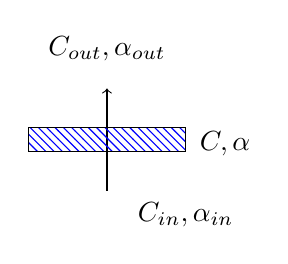
\begin{tikzpicture}
        \coordinate (1) at (0, 1);
        \coordinate (2) at (0, 2.3);
        \coordinate (3) at (0, 2.8);
        \eye{0.5}{0}{0}{90};
        \draw[->] (1) -- (2);
        \node at (1, 0.7) {$C_{in}, \alpha_{in}$};
        \node at (3) {$C_{out}, \alpha_{out}$};

        \draw[pattern=north west lines, pattern color=blue] (-1, 1.8) rectangle (1, 1.5);
        \node at (1.5, 1.6) {$C, \alpha$};
    \end{tikzpicture}
\end{center}

\subsection{Direct Volume Rendering: Phong Shading}
We have to evaluate Phong's illumination model based on: \\
$\bullet$ \textbf{position} of current sample and light source \\
$\bullet$ sample's \textnormal{color} emission assigned by transfer function \\
$\bullet$ sample's \textbf{normal/gradient} (central difference)

\subsection{Gradient Estimation}
We can estimate the gradient using finite differencing. However, this technique is not feasible with large amounts of data.

\begin{align*}
    & \nabla f(x, y, z) \approx \\
    & \approx \frac{1}{2h} \begin{pmatrix}
        f(x + h, y, z) - f(x - h, y, z) \\
        f(x, y + h, z) - f(x, y - h, z) \\
        f(x, y, z + h) - f(x, y, z - h) \\
    \end{pmatrix}
\end{align*}

\subsection{Compositing Schemes}
$\bullet$ \textbf{Surface Rendering/First-Hit}: stop ray traversal if an ISOSurface is hit \\
$\bullet$ \textbf{Average}: simply accumulate colors, but ignore opacity \\
$\bullet$ \textbf{Maximum}: take maximum color along axis and display it
\section{Flow Visualization}
$\bullet$ Motion of fluids (gases, liquids) \\
$\bullet$ Geometric boundaries \\
$\bullet$ Conservation of mass, energy and momentum \\
$\bullet$ Velocity/Flow field $v(x, t)$

\subsection{Vector Field Visualization}
$\bullet$ Vector data representing \textbf{Direction} and \textbf{Magnitude} \\
$\bullet$ \textbf{Steady} (time-indipendent) flow:
$$v(x): \mathbb{R}^n \rightarrow \mathbb{R}^n$$
$\bullet$ \textbf{Unsteady} (time dependent) flow:
$$v(x, t): \mathbb{R}^n \times \mathbb{R}^1 \rightarrow \mathbb{R}^n$$


\subsection{Vector and Scalar Functions}
Scalar function:
$$\rho(x, t)$$
The gradient points to the direction of maximum change of $\rho (x, t)$:
$$\nabla \rho(x, t) = \Scale[1.3]{\begin{pmatrix}
            \frac{\delta \rho(x, t)}{\delta x} \\
            \frac{\delta \rho(x, t)}{\delta y} \\
            \frac{\delta \rho(x, t)}{\delta z} \\
        \end{pmatrix}}$$

Jacobian matrix applied to vector field $v(x, t)$:
$$J = \nabla v(x, t) = \Scale[1.2]{\begin{pmatrix}
            \tcbhighmath[myinner, colback=orange!50!white]{\frac{\delta v_x}{\delta x}} & \tcbhighmath[myinner, colback=blue!20!white]{\frac{\delta v_x}{\delta y}}   & \tcbhighmath[myinner, colback=violet!20!white]{\frac{\delta v_x}{\delta z}} \\
            %
            \tcbhighmath[myinner, colback=blue!20!white]{\frac{\delta v_y}{\delta x}}   & \tcbhighmath[myinner, colback=orange!50!white]{\frac{\delta v_y}{\delta y}} & \tcbhighmath[myinner, colback=green!20!white]{\frac{\delta v_y}{\delta z}}  \\
            %
            \tcbhighmath[myinner, colback=violet!20!white]{\frac{\delta v_z}{\delta x}} & \tcbhighmath[myinner, colback=green!20!white]{\frac{\delta v_z}{\delta y}}  & \tcbhighmath[myinner, colback=orange!50!white]{\frac{\delta v_z}{\delta z}} \\
        \end{pmatrix}}$$

\textbf{Divergence}: Diagonal of Jacobian, describes flow into/out of a region:
$$div\ v(x, t) = \tcbhighmath[myinner, colback=orange!50!white]{\frac{\delta v_x}{\delta x} + \frac{\delta v_y}{\delta y} + \frac{\delta v_z}{\delta z}}$$
\begin{align*}
    div\ v(x_0) > 0 & : v\text{ has \textbf{source} in } x_0     \\
    div\ v(x_0) < 0 & : v\text{ has \textbf{sink} in } x_0       \\
    div\ v(x_0) = 0 & : v\text{ is \textbf{source-free} in } x_0 \\
\end{align*}

\textbf{Curl/vorticity}: tells how fast the flow is rotating, and the axis around which it is rotating.
$$curl\ v(x, t) = \nabla v(x, t) = \begin{pmatrix}
        \tcbhighmath[myinner, colback=green!20!white]{\frac{\delta v_z}{\delta y} - \frac{\delta v_y}{\delta z}}  \\
        \tcbhighmath[myinner, colback=violet!20!white]{\frac{\delta v_x}{\delta z} - \frac{\delta v_z}{\delta x}} \\
        \tcbhighmath[myinner, colback=blue!20!white]{\frac{\delta v_y}{\delta x} - \frac{\delta v_x}{\delta y}}
    \end{pmatrix}$$

\subsection{Computing Characteristic Lines}
Characteristic lines are \textbf{tangential} to the flow.

$$\frac{\delta x(t)}{\delta t} = v(x(t), t)$$

$\bullet$ do not intersect \\
$\bullet$ they are the solutions to the initial value problem

\subsection{Euler Method}
$\bullet$ First order method \\
$\bullet$ higher accuracy with smaller step size ($\Delta t$)

$$x(t + \Delta t) \approx  x(t) + \Delta t \cdot v(x(t), t)$$

\subsection{Midpoint Method}
$\bullet$ Better, faster than Euler method

\begin{align*}
    \Delta x        & = \Delta t \cdot v(x, t)                            \\
    v_{mid}         & = v(x + \frac{\Delta x}{2}, t + \frac{\Delta t}{2}) \\
    x(t + \Delta t) & = x(t) + \Delta t \cdot v_{mid}
\end{align*}

\subsection{Runge-Kutta 4th Order}
$\bullet$ The most accurate

\begin{align*}
    k_1             & = \Delta t \cdot v(x, t)                                            \\
    k_2             & = \Delta t \cdot v(x + \frac{k_1}{2}, t + \frac{\Delta t}{2})       \\
    k_3             & = \Delta t \cdot v(x + \frac{k_2}{2}, t + \frac{\Delta t}{2})       \\
    k_4             & = \Delta t \cdot v(x + k_3, t + \frac{\Delta t}{2})                 \\
    x(t + \Delta t) & = k + \frac{k_1}{6} + \frac{k_2}{3} + \frac{k_3}{3} + \frac{k_4}{6}
\end{align*}

\subsection{Vector Field Topology}
$\bullet$ We want ot draw along the most important lines \\
$\bullet$ Draw topological skeleton of flow \\

\subsection{Critical Points}
$\bullet$ Singularities in vector fields such that: \\
$$v(x^*) = 0$$
$\bullet$ Points where magnitude of veectors goes to zero and direction of vectors is undefined \\

\textbf{To find critical points}: points where:
$$v(x^*) = 0$$

\textbf{Classification}
First, we build the Jacobian matrix for $v(x^*)$

$$J = \Scale[1.3]{\begin{pmatrix}
            \frac{\delta v_x}{\delta x} & \frac{\delta v_x}{\delta y} \\
            \frac{\delta v_y}{\delta x} & \frac{\delta v_y}{\delta y} \\
        \end{pmatrix}}$$

Then, for each $x^*$ calculate the \textbf{eigenvalues} $\lambda_1, \lambda_2$ of $J$. \\
To find the eigen values:

$$det(J - \lambda I) = det\Scale[1.3]{\begin{pmatrix}
            \frac{\delta v_x}{\delta x} - \lambda & \frac{\delta v_x}{\delta y}           \\
            \frac{\delta v_y}{\delta x}           & \frac{\delta v_y}{\delta y} - \lambda \\
        \end{pmatrix}}$$

\begin{align*}
     & \text{\textbf{Circulating Source}}                                        \\
     & Im(\lambda_1, \lambda_2) \neq 0 \text{ and } Re(\lambda_1, \lambda_2) > 0 \\
     & \text{\textbf{Non-Circulating Source}}                                    \\
     & Im(\lambda_1, \lambda_2) = 0 \text{ and } Re(\lambda_1, \lambda_2) > 0    \\
     & \text{\textbf{Center}}                                                    \\
     & Im(\lambda_1, \lambda_2) \neq 0 \text{ and } Re(\lambda_1, \lambda_2) = 0 \\
     & \text{\textbf{Circulating Sink}}                                          \\
     & Im(\lambda_1, \lambda_2) \neq 0 \text{ and } Re(\lambda_1, \lambda_2) < 0 \\
     & \text{\textbf{Non-Circulating Sink}}                                      \\
     & Im(\lambda_1, \lambda_2) = 0 \text{ and } Re(\lambda_1, \lambda_2) < 0    \\
     & \text{\textbf{Saddle Point}}                                              \\
     & Im(\lambda_1, \lambda_2) = 0 \text{ and } \lambda_1 \cdot \lambda_2 < 0   \\
\end{align*}

\subsection{Dense Texture-Based Flow Visualization}
$\bullet$ Better information coverage \\
$\bullet$ Critical point detection and classification \\

\subsection{Line-Integral Convolution}
$\bullet$ Global visualization technique \\
$\bullet$ Starts with random noise (white noise) \\
$\bullet$ \textit{Smear out} the texture along trajectories of vector field \\
$\bullet$  Results in \textbf{low correlation} between \textbf{neighbouring lines} and \textbf{high correlation} along \textbf{flow direction} \\

Steps: \\
$\bullet$ Vector Field $\rightarrow$ (integration) Stream Line \\
$\bullet$ Stream Line $\rightarrow$ (convolution) Noise Texture \\
$\bullet$ Noise Texture $\rightarrow$ (result) Output Image \\

\subsection{Filtering By Convolution}
$\bullet$ Sliding a function $g(x)$ along a function $f(x)$:

$$s(x') = [f * g](x') = \int_{-\infty}^{\infty} f(x) g(x' - x) \,dx$$

$\bullet$ Function $f$ is averaged with a weight function $g$ \\
$\bullet$ $(x' - x)$ centers $g$ around $x'$ \\

$\bullet$ We use the single stream lines that pass through a single pixel to smear out the noise \\
$\bullet$ $\varPhi_0 (u)$ is the stream line containing the point $(x_0, y_0)$ \\
$\bullet$ $T(x, y)$ is the randomly generated noise texture \\
$\bullet$ Compute the intensity at $(x_0, y_0)$ as: \\
$$I(x_0, y_0) = \int_{-L}^{L} k(u) \cdot T(\varPhi(u)) \,du$$


\end{multicols}

\end{document}
